\documentclass[
  11pt,
  letterpaper,
   addpoints,
   answers
  ]{exam}

\usepackage{../exercise-preamble}
\usepackage{float}
% TikZ libraries needed for `right=.. of ..` and coordinate math
\usetikzlibrary{positioning,calc,arrows,arrows.meta}
% Alias de seguridad por si se escribe 'ikzstyle' por error
\let\ikzstyle\tikzstyle

\begin{document}

\noindent
\begin{minipage}{0.47\textwidth}
\includegraphics[width=\textwidth]{../fcfm_die}
\end{minipage}
\begin{minipage}{0.53\textwidth}
\begin{center} 
\large\textbf{Análisis de señales} (EL3203-2) \\
\large\textbf{Pauta Tarea 3} \\
\normalsize Prof.~Jorge Silva.\\
\normalsize Prof.~Aux.~Erik Sáez
\end{center}
\end{minipage}

\vspace{0.5cm}
\noindent
\vspace{.85cm}

\begin{questions}
    %%%%%%%%%%%%%%%%%%%%%%%%%%%
\question \textbf{[2 Puntos]} Pregunta 1
\begin{enumerate}
    \item[(a)] \textbf{[0.5 Puntos]} Sea $(x(n))_{n \in \mathbb{Z}}$ una señal discreta de energía finita con \textbf{Transformada de Fourier} $X(w)$ definida en $w \in [0, 2\pi)$. Considere la extensión $N$-periódica de $x(n)$ dada por:
    \[
    x_N(n) = \sum_{l \in \mathbb{Z}} x(n - l \cdot N), \quad \forall n \in \mathbb{Z}.
    \]
    
    Verifique que los coeficientes de la \textbf{Serie de Fourier} de $(x_N(n))$, es decir $\{c_k^N : k = 0, \ldots, N-1\}$, se obtienen por medio del muestreo uniforme de $X(w)$. En particular, verifique que:
    \[
    c_k^N = \frac{1}{N} X\left(\frac{2\pi k}{N}\right), \quad \forall k \in \{0, \ldots, N-1\}.
    \]
    
    \begin{solution}
    Los coeficientes de la Serie de Fourier de $x_N(n)$ están dados por:
    \[
    c_k^N = \frac{1}{N} \sum_{n=0}^{N-1} x_N(n) e^{-j \frac{2\pi k n}{N}}
    \]
    
    Sustituyendo la definición de $x_N(n)$:
    \[
    c_k^N = \frac{1}{N} \sum_{n=0}^{N-1} \left[\sum_{l \in \mathbb{Z}} x(n - l \cdot N)\right] e^{-j \frac{2\pi k n}{N}}
    \]
    
    Intercambiando el orden de las sumatorias:
    \[
    c_k^N = \frac{1}{N} \sum_{l \in \mathbb{Z}} \sum_{n=0}^{N-1} x(n - l \cdot N) e^{-j \frac{2\pi k n}{N}}
    \]
    
    Haciendo el cambio de variable $m = n - l \cdot N$, cuando $n$ recorre $\{0, 1, \ldots, N-1\}$ para un $l$ fijo, $m$ recorre $\{-l \cdot N, -l \cdot N + 1, \ldots, -l \cdot N + N - 1\}$. Entonces:
    \[
    c_k^N = \frac{1}{N} \sum_{l \in \mathbb{Z}} \sum_{m=-l \cdot N}^{-l \cdot N + N - 1} x(m) e^{-j \frac{2\pi k (m + l \cdot N)}{N}}
    \]
    
    Expandiendo el exponente:
    \[
    e^{-j \frac{2\pi k (m + l \cdot N)}{N}} = e^{-j \frac{2\pi k m}{N}} \cdot e^{-j \frac{2\pi k l \cdot N}{N}} = e^{-j \frac{2\pi k m}{N}} \cdot e^{-j 2\pi k l}
    \]
    Notemos que $e^{-j 2\pi k l} = 1$ para todo $k, l \in \mathbb{Z}$.Esto se debe a que $2\pi k l$ es siempre un múltiplo entero de $2\pi$, y la función exponencial compleja tiene período $2\pi$. Por lo tanto:
    \[
    c_k^N = \frac{1}{N} \sum_{l \in \mathbb{Z}} \sum_{m=-l \cdot N}^{-l \cdot N + N - 1} x(m) e^{-j \frac{2\pi k m}{N}}
    \]
     Al sumar sobre todos los enteros $l \in \mathbb{Z}$, los intervalos $[-l \cdot N, -l \cdot N + N - 1]$ cubren todo $\mathbb{Z}$ sin traslapes. Para ver esto:
    
    \begin{itemize}
        \item Para $l = 0$: el intervalo es $[0, N-1]$
        \item Para $l = 1$: el intervalo es $[-N, -1]$
        \item Para $l = -1$: el intervalo es $[N, 2N-1]$
        \item Para $l = 2$: el intervalo es $[-2N, -N-1]$
        \item Y así sucesivamente...
    \end{itemize}
    
    Por lo tanto, podemos reescribir la doble suma como una suma simple sobre todos los enteros:
    \[
    c_k^N = \frac{1}{N} \sum_{m \in \mathbb{Z}} x(m) e^{-j \frac{2\pi k m}{N}}
    \]
    
    Ahora, observemos que la expresión que obtuvimos para $c_k^N$ tiene una forma muy similar a la Transformada de Fourier en tiempo discreto (DTFT).Recordemos que la DTFT de una señal $x(m)$ se define como:
    \[
    X(w) = \sum_{m \in \mathbb{Z}} x(m) e^{-j w m}
    \]
    
    donde $w$ es la frecuencia angular (una variable continua).Ahora, comparemos esta definición con lo que tenemos en $c_k^N$:
    \[
    c_k^N = \frac{1}{N} \sum_{m \in \mathbb{Z}} x(m) e^{-j \frac{2\pi k m}{N}}
    \]
    
    Si hacemos la sustitución $w = \frac{2\pi k}{N}$ en la definición de $X(w)$, obtenemos:
    \[
    X\left(\frac{2\pi k}{N}\right) = \sum_{m \in \mathbb{Z}} x(m) e^{-j \frac{2\pi k}{N} \cdot m} = \sum_{m \in \mathbb{Z}} x(m) e^{-j \frac{2\pi k m}{N}}
    \]
  
    Por lo tanto, podemos identificar:
    \[
    \sum_{m \in \mathbb{Z}} x(m) e^{-j \frac{2\pi k m}{N}} = X\left(\frac{2\pi k}{N}\right)
    \]
    
    Sustituyendo esto en nuestra expresión para $c_k^N$:
    \[
    \boxed{c_k^N = \frac{1}{N} X\left(\frac{2\pi k}{N}\right)}
    \]
    
    \end{solution}
    
    \item[(b)] \textbf{[0.5 Puntos]} Continuando el punto anterior, obtenga una expresión para el centro de masa de $(x(n))_{n \in \mathbb{Z}}$, i.e.,
    \[
    c \equiv \frac{\sum_{n \in \mathbb{Z}} n \cdot x(n)}{\sum_{n \in \mathbb{Z}} x(n)},
    \]
    como función de $X(w)$.
    
    \begin{solution}
    Del resultado de la parte (a), sabemos que:
    \[
    c_k^N = \frac{1}{N} X\left(\frac{2\pi k}{N}\right)
    \]
    Queremos calcular el centro de masa de la señal aperiódica original $x(n)$:
    \[
    c = \frac{\sum_{n \in \mathbb{Z}} n \cdot x(n)}{\sum_{n \in \mathbb{Z}} x(n)}
    \]
    
    Para esto, necesitamos expresar el numerador y denominador en términos de la Transformada de Fourier $X(w)$.
  
    
    El denominador es simplemente la suma de todos los valores de $x(n)$. Recordemos la definición de la Transformada de Fourier:
    \[
    X(w) = \sum_{n \in \mathbb{Z}} x(n) e^{-j w n}
    \]
    
    Si evaluamos esta expresión en $w = 0$:
    \[
    X(0) = \sum_{n \in \mathbb{Z}} x(n) e^{-j \cdot 0 \cdot n} = \sum_{n \in \mathbb{Z}} x(n) \cdot 1 = \sum_{n \in \mathbb{Z}} x(n)
    \]
     Porque $e^0 = 1$, lo que hace desaparecer la exponencial compleja y nos queda exactamente la suma que necesitamos. Por lo tanto:
    \[
    \boxed{\sum_{n \in \mathbb{Z}} x(n) = X(0)}
    \]
    
    Para el numerador, necesitamos calcular $\sum_{n \in \mathbb{Z}} n \cdot x(n)$. Aquí utilizaremos una propiedad importante de la Transformada de Fourier.Si derivamos la Transformada de Fourier respecto a $w$:
    \[
    \frac{dX(w)}{dw} = -j \sum_{n \in \mathbb{Z}} n \cdot x(n) e^{-j w n}
    \]
    
    Ahora, \textbf{evaluamos en $w = 0$}:
    \[
    \left.\frac{dX(w)}{dw}\right|_{w=0} = -j \sum_{n \in \mathbb{Z}} n \cdot x(n) e^{-j \cdot 0 \cdot n} = -j \sum_{n \in \mathbb{Z}} n \cdot x(n)
    \]
    
    Sustituyendo ambos resultados en la definición del centro de masa:
    \[
    c = \frac{\sum_{n \in \mathbb{Z}} n \cdot x(n)}{\sum_{n \in \mathbb{Z}} x(n)} = \frac{j \frac{dX(w)}{dw}\big|_{w=0}}{X(0)}
    \]
    
    Simplificando:
    \[
    c = \frac{j}{X(0)} \cdot \left.\frac{dX(w)}{dw}\right|_{w=0}
    \]
    
    Alternativamente, usando la notación $X'(w) = \frac{dX(w)}{dw}$:
    \[
    \boxed{c = -j \frac{X'(0)}{X(0)}}
    \]
  
    \end{solution}
    
    \item[(c)] \textbf{[0.5 Puntos]} Sea $(\psi_f(n)) = (e^{j 2 \pi f n})_{n \in \mathbb{Z}}$ la familia de señales sinusoidales complejas indexadas por $f \in (-1/2, 1/2]$. Muestre que todo \textbf{Sistema LTI} estable de respuesta al impulso $(h(n))_{n \in \mathbb{Z}}$ cumple que:
    \[
    (\psi_f(n)) * (h(n)) = \lambda_f \cdot (\psi_f(n)).
    \tag{1}
    \]
    
    Determine una expresión para el valor $\lambda_f$ y comente el resultado.
    
    \begin{solution}
    Calculemos la convolución de $\psi_f(n)$ con $h(n)$:
    \[
    y(n) = (\psi_f(n)) * (h(n)) = \sum_{m \in \mathbb{Z}} \psi_f(m) \cdot h(n-m)
    \]
    
    Sustituyendo $\psi_f(m) = e^{j 2\pi f m}$:
    \[
    y(n) = \sum_{m \in \mathbb{Z}} e^{j 2\pi f m} \cdot h(n-m)
    \]
    
    Haciendo el cambio de variable $k = n - m$, entonces $m = n - k$:
    \[
    y(n) = \sum_{k \in \mathbb{Z}} e^{j 2\pi f (n-k)} \cdot h(k) = e^{j 2\pi f n} \sum_{k \in \mathbb{Z}} e^{-j 2\pi f k} \cdot h(k)
    \]
    
    Observamos que:
    \[
    y(n) = e^{j 2\pi f n} \cdot H(2\pi f) = \psi_f(n) \cdot H(2\pi f)
    \]
    
    donde $H(w) = \sum_{k \in \mathbb{Z}} h(k) e^{-j w k}$ es la respuesta en frecuencia del sistema.
    
    Por lo tanto:
    \[
    \lambda_f = H(2\pi f)
    \]
    
    \end{solution}
    
    \item[(d)] \textbf{[0.5 Puntos]} Considere $(x(n))_{n \in \mathbb{Z}}$ una señal discreta $N$-periódica a la entrada de un sistema LTI estable de respuesta al impulso $(h(n))_{n \in \mathbb{Z}}$.
    
    \begin{itemize}
        \item Demuestre que $(y(n)) = (x(n)) * (h(n))$ es $N$-periódica.
        \item Encuentre la relación entre los coeficientes de la \textbf{Serie de Fourier} de la salida $(y(n))$ y la entrada $(x(n))$.
        \item Determine el operador equivalente del sistema LTI en el dominio de las \textbf{Series de Fourier} de señales $N$-periódicas y verifique que es una matriz diagonal.
    \end{itemize}
    
    \begin{solution}
 Para demostrar que $y(n)$ es $N$-periódica, debemos mostrar que $y(n+N) = y(n)$ para todo $n \in \mathbb{Z}$. Como $x(n)$ es $N$-periódica, podemos escribirla usando su Serie de Fourier:
    \[
    x(n) = \sum_{k=0}^{N-1} c_k e^{j \frac{2\pi k n}{N}}
    \]
    
    donde $c_k$ son los coeficientes de la Serie de Fourier de $x(n)$. La salida del sistema LTI es la convolución:
    \[
    y(n) = x(n) * h(n) = \sum_{m \in \mathbb{Z}} x(m) h(n-m)
    \]
    
    Sustituyendo la Serie de Fourier de $x(n)$:
    \[
    y(n) = \sum_{m \in \mathbb{Z}} \left[\sum_{k=0}^{N-1} c_k e^{j \frac{2\pi k m}{N}}\right] h(n-m)
    \]
    
    Intercambiando las sumatorias (los $c_k$ son constantes):
    \[
    y(n) = \sum_{k=0}^{N-1} c_k \sum_{m \in \mathbb{Z}} e^{j \frac{2\pi k m}{N}} h(n-m)
    \]
     Reconocemos que la suma interna es una convolución de la exponencial compleja $e^{j \frac{2\pi k m}{N}}$ con $h(n)$.
    
    Aplicando el resultado de la parte (c) con $f = \frac{k}{N}$, sabemos que las exponenciales complejas son eigenfunciones de sistemas LTI:
    \[
    \sum_{m \in \mathbb{Z}} e^{j \frac{2\pi k m}{N}} h(n-m) = H\left(\frac{2\pi k}{N}\right) e^{j \frac{2\pi k n}{N}}
    \]
    
    Por lo tanto:
    \[
    y(n) = \sum_{k=0}^{N-1} c_k H\left(\frac{2\pi k}{N}\right) e^{j \frac{2\pi k n}{N}}
    \]
    
    La expresión anterior es una Serie de Fourier de la forma:
    \[
    y(n) = \sum_{k=0}^{N-1} d_k e^{j \frac{2\pi k n}{N}}
    \]
    
    donde $d_k = c_k H\left(\frac{2\pi k}{N}\right)$.
    
    Esta es la definición estándar de una Serie de Fourier discreta con período $N$. Para verificar la periodicidad, evaluemos $y(n+N)$:
    \[
    y(n+N) = \sum_{k=0}^{N-1} d_k e^{j \frac{2\pi k (n+N)}{N}} = \sum_{k=0}^{N-1} d_k e^{j \frac{2\pi k n}{N}} \cdot e^{j 2\pi k}
    \]
    
    Como $e^{j 2\pi k} = 1$ para todo $k \in \mathbb{Z}$:
    \[
    y(n+N) = \sum_{k=0}^{N-1} d_k e^{j \frac{2\pi k n}{N}} = y(n)
    \]
  
    \vspace{0.3cm}
    \textbf{Segunda parte: Relación entre coeficientes}
    
    Sean $d_k$ los coeficientes de la Serie de Fourier de $y(n)$:
    \[
    y(n) = \sum_{k=0}^{N-1} d_k e^{j \frac{2\pi k n}{N}}
    \]
    
    Comparando con la expresión obtenida anteriormente:
    \[
    d_k = c_k \cdot H\left(\frac{2\pi k}{N}\right), \quad k = 0, 1, \ldots, N-1
    \]
    
    Es decir, cada coeficiente de Fourier de la salida se obtiene multiplicando el coeficiente correspondiente de la entrada por la respuesta en frecuencia evaluada en esa frecuencia particular.
    
    \vspace{0.3cm}
    \textbf{Tercera parte: Operador equivalente}
    
    Podemos representar las señales $N$-periódicas mediante vectores de sus coeficientes de Fourier:
    \[
    \mathbf{c} = \begin{bmatrix} c_0 \\ c_1 \\ \vdots \\ c_{N-1} \end{bmatrix}, \quad
    \mathbf{d} = \begin{bmatrix} d_0 \\ d_1 \\ \vdots \\ d_{N-1} \end{bmatrix}
    \]
    
    La relación entre entrada y salida es:
    \[
    \mathbf{d} = \mathbf{H} \cdot \mathbf{c}
    \]
    
    donde $\mathbf{H}$ es una matriz diagonal:
    \[
    \mathbf{H} = \begin{bmatrix}
    H\left(\frac{2\pi \cdot 0}{N}\right) & 0 & \cdots & 0 \\
    0 & H\left(\frac{2\pi \cdot 1}{N}\right) & \cdots & 0 \\
    \vdots & \vdots & \ddots & \vdots \\
    0 & 0 & \cdots & H\left(\frac{2\pi (N-1)}{N}\right)
    \end{bmatrix}
    \]
    
    Podemos escribir:
    \[
    \mathbf{H} = \text{diag}\left(H(0), H\left(\frac{2\pi}{N}\right), H\left(\frac{4\pi}{N}\right), \ldots, H\left(\frac{2\pi(N-1)}{N}\right)\right)
    \]
    
    Esta matriz es diagonal porque cada coeficiente de Fourier de la salida depende únicamente del coeficiente correspondiente de la entrada, sin acoplamiento entre diferentes frecuencias. Esto refleja la propiedad fundamental de que los sistemas LTI procesan cada componente de frecuencia de manera independiente.
    \end{solution}
\end{enumerate}

%%%%%%%%%%%%%%%%%%%%%%%%%%%
\question
Considerando que la señal $(x(n))_{n\in\mathbb{Z}}$ y su \textbf{Transformada de Fourier} $X(\omega)$ están dadas por las expresiones:
\[
x(n) = \begin{cases}
1 & -M \leq n \leq M \\
0 & \text{en otro caso}
\end{cases}
\]
\[
X(\omega) = 1 + 2\sum_{n=1}^{M} \cos(\omega n)
\]

Demuestre que las \textbf{Transformadas de Fourier} de:
\[
x_1(n) = \begin{cases}
1 & 0 \leq n \leq M \\
0 & \text{en otro caso}
\end{cases}
\]

y
\[
x_2(n) = \begin{cases}
1 & -M \leq n \leq -1 \\
0 & \text{en otro caso}
\end{cases}
\]

son respectivamente,
\[
X_1(\omega) = \frac{1 - e^{-j\omega(M+1)}}{1 - e^{-j\omega}}
\]

y
\[
X_2(\omega) = \frac{e^{j\omega} - e^{j\omega(M+1)}}{1 - e^{j\omega}}.
\]

Concluya finalmente que
\[
X(\omega) = X_1(\omega) + X_2(\omega) = \frac{\sin(M + \frac{1}{2})\omega}{\sin(\omega/2)}
\]

y por consiguiente que
\[
1 + 2\sum_{n=1}^{M} \cos(\omega n) = \frac{\sin(M + \frac{1}{2})\omega}{\sin(\omega/2)}.
\]

\begin{solution}
Sea
\[
x[n]=
\begin{cases}
1, & -M\le n\le M,\\
0, & \text{en otro caso},
\end{cases}
\qquad M\in\mathbb{Z}_{\ge 0}.
\]
La DTFT de $x[n]$ puede escribirse (por simetría par) como
\[
X(\omega)=\sum_{n=-M}^{M}e^{-j\omega n}=1+2\sum_{n=1}^{M}\cos(\omega n).
\]
Se pide: \textbf{(i)} demostrar las DTFT de las señales truncadas hacia la derecha e izquierda, y \textbf{(ii)} concluir una forma cerrada para $X(\omega)$.
Definimos las señales truncadas:
\begin{align*}
x_1[n] &= \begin{cases}
1, & 0 \leq n \leq M, \\
0, & \text{en otro caso},
\end{cases} \\
x_2[n] &= \begin{cases}
1, & -M \leq n \leq -1, \\
0, & \text{en otro caso}.
\end{cases}
\end{align*}

Observemos que $x[n] = x_1[n] + x_2[n] + \delta[n]$, donde $\delta[n]$ es el impulso unitario en $n=0$.

\textbf{Cálculo de $X_1(\omega)$:}

Por definición de la DTFT:
\begin{align*}
X_1(\omega) &= \sum_{n=-\infty}^{\infty} x_1[n]e^{-j\omega n} = \sum_{n=0}^{M}e^{-j\omega n} \\
&= 1+e^{-j\omega}+e^{-j2\omega}+\cdots+e^{-jM\omega}.
\end{align*}

Esta es una serie geométrica con primer término $a=1$, razón $r=e^{-j\omega}$ y $M+1$ términos:
\[
X_1(\omega) = \frac{1 - (e^{-j\omega})^{M+1}}{1 - e^{-j\omega}} = \frac{1 - e^{-j\omega(M+1)}}{1 - e^{-j\omega}}.
\]

\textbf{Cálculo de $X_2(\omega)$:}

Análogamente, para la señal truncada hacia la izquierda:
\begin{align*}
X_2(\omega) &= \sum_{n=-\infty}^{\infty} x_2[n]e^{-j\omega n} = \sum_{n=-M}^{-1}e^{-j\omega n}.
\end{align*}

Con el cambio de variable $n=-(m+1)$ donde $m=0,1,\ldots,M-1$:
\begin{align*}
X_2(\omega) &= \sum_{m=0}^{M-1}e^{-j\omega(-m-1)} = \sum_{m=0}^{M-1}e^{j\omega(m+1)} \\
&= e^{j\omega}\sum_{m=0}^{M-1}e^{j\omega m} = e^{j\omega}\,\frac{1-e^{j\omega M}}{1-e^{j\omega}} \\
&= \frac{e^{j\omega}-e^{j\omega(M+1)}}{1-e^{j\omega}}.
\end{align*}

Por tanto:
\[
\boxed{
X_1(\omega) = \frac{1-e^{-j\omega(M+1)}}{1-e^{-j\omega}}, \quad
X_2(\omega) = \frac{e^{j\omega}-e^{j\omega(M+1)}}{1-e^{j\omega}}
}
\]

\subsection*{Parte (ii): Forma cerrada de $X(\omega)$}

La señal original se reconstruye como:
\[
X(\omega) = X_1(\omega) + X_2(\omega)
\]

Sustituyendo las expresiones obtenidas:
\begin{align*}
X(\omega) &= \frac{1-e^{-j\omega(M+1)}}{1-e^{-j\omega}} + \frac{e^{j\omega}-e^{j\omega(M+1)}}{1-e^{j\omega}}
\end{align*}

Para sumar estas fracciones, necesitamos un denominador común. Observemos que:
\[
\frac{1-e^{-j\omega(M+1)}}{1-e^{-j\omega}} = \frac{e^{j\omega(M+1)}-1}{e^{j\omega}-1}
\]

Multiplicando numerador y denominador de la primera fracción por $e^{j\omega(M+1)}$ y usando $e^{j\omega}(1-e^{-j\omega}) = e^{j\omega}-1$:

\begin{align*}
X(\omega) &= \frac{e^{j\omega(M+1)}-1}{e^{j\omega}-1} + \frac{e^{j\omega}-e^{j\omega(M+1)}}{1-e^{j\omega}} \\
&= \frac{e^{j\omega(M+1)}-1}{e^{j\omega}-1} - \frac{e^{j\omega}-e^{j\omega(M+1)}}{e^{j\omega}-1} \\
&= \frac{e^{j\omega(M+1)}-1 - e^{j\omega} + e^{j\omega(M+1)}}{e^{j\omega}-1} \\
&= \frac{2e^{j\omega(M+1)} - e^{j\omega} - 1}{e^{j\omega}-1}
\end{align*}

Factorizando $e^{j\omega(M+1/2)}$ en el numerador y $e^{j\omega/2}$ en el denominador:
\[
X(\omega) = \frac{e^{j\omega(M+1/2)}(e^{j\omega/2} - e^{-j\omega/2}) + e^{j\omega(M+1/2)}(e^{j\omega/2} - e^{-j\omega/2})}{e^{j\omega/2}(e^{j\omega/2} - e^{-j\omega/2})}
\]

Simplificando con $e^{j\theta} - e^{-j\theta} = 2j\sin(\theta)$:
\[
X(\omega) = \frac{e^{j\omega(M+1/2)} - e^{-j\omega(M+1/2)}}{e^{j\omega/2} - e^{-j\omega/2}} = \frac{2j\sin\left((M+\tfrac{1}{2})\omega\right)}{2j\sin(\omega/2)} = \frac{\sin\left((M+\tfrac{1}{2})\omega\right)}{\sin(\omega/2)}
\]

La expresión en cosenos se obtiene por la simetría par de $x[n]$:
\begin{align*}
X(\omega) &= \sum_{n=-M}^{M}e^{-j\omega n} = e^{-j\omega M} + e^{-j\omega(M-1)} + \cdots + 1 + \cdots + e^{j\omega M} \\
&= 1 + 2\sum_{n=1}^{M}\cos(\omega n)
\end{align*}

Por tanto, ambas formas son equivalentes:
\[
\boxed{
1+2\sum_{n=1}^{M}\cos(\omega n) = \frac{\sin\left((M+\tfrac{1}{2})\omega\right)}{\sin(\omega/2)}
}
\]

Esta identidad corresponde al \textit{núcleo de Dirichlet} y es fundamental en análisis de Fourier. La expresión es válida para todo $\omega \neq 2\pi k$ con $k \in \mathbb{Z}$. En los puntos $\omega = 2\pi k$, el límite da $X(2\pi k) = 2M+1$, que es el número total de muestras no nulas de $x[n]$.
\end{solution}

%%%%%%%%%%%%%%%%%%%%%%%%%%%
\question \textbf{[2 Puntos]} Pregunta 3
\begin{enumerate}
    \item[(i)] \textbf{[1.5 Puntos]} Para los distintos casos ilustrados en las Figuras \ref{fig:q3a}, \ref{fig:q3b}, \ref{fig:q3c} y \ref{fig:q3d}, determine las señales $(x(n))_{n\in\mathbb{Z}}$ a partir de sus respectivas \textbf{Transformadas de Fourier}.

\begin{figure}[H]
\centering
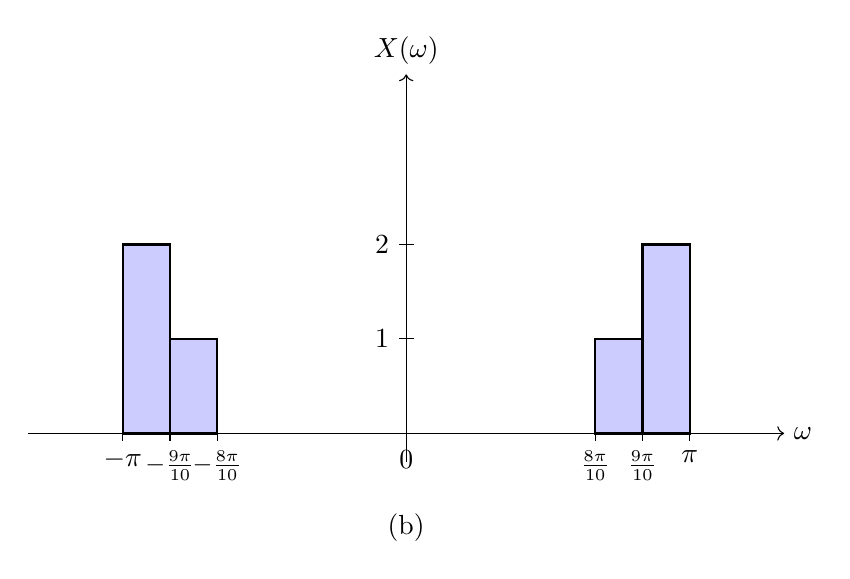
\begin{tikzpicture}[scale=1.2]
% Ejes
\draw[->] (-4,0) -- (4,0) node[right] {$\omega$};
\draw[->] (0,-0.3) -- (0,3.8) node[above] {$X(\omega)$};

% Marcas en el eje x
\draw (-3,0.08) -- (-3,-0.08) node[below] {$-\pi$};
\draw (-2.5,0.08) -- (-2.5,-0.08) node[below,font=\small] {$-\frac{9\pi}{10}$};
\draw (-2,0.08) -- (-2,-0.08) node[below,font=\small] {$-\frac{8\pi}{10}$};
\draw (0,0.08) -- (0,-0.08) node[below] {$0$};
\draw (2,0.08) -- (2,-0.08) node[below,font=\small] {$\frac{8\pi}{10}$};
\draw (2.5,0.08) -- (2.5,-0.08) node[below,font=\small] {$\frac{9\pi}{10}$};
\draw (3,0.08) -- (3,-0.08) node[below] {$\pi$};

% Marcas en el eje y
\draw (0.08,1) -- (-0.08,1) node[left] {$1$};
\draw (0.08,2) -- (-0.08,2) node[left] {$2$};

% Región izquierda: de -π a -9π/10 (altura 2)
\draw[thick,fill=blue!20] (-3,0) rectangle (-2.5,2);

% Región: de -9π/10 a -8π/10 (altura 1)
\draw[thick,fill=blue!20] (-2.5,0) rectangle (-2,1);

% Región: de 8π/10 a 9π/10 (altura 1)
\draw[thick,fill=blue!20] (2,0) rectangle (2.5,1);

% Región derecha: de 9π/10 a π (altura 2)
\draw[thick,fill=blue!20] (2.5,0) rectangle (3,2);

% Etiqueta (b)
\node at (0,-1) {(b)};

\end{tikzpicture}
\caption{Transformada de Fourier $X(\omega)$ -- Caso (b)}
\label{fig:q3b}
\end{figure}

\begin{figure}[H]
\centering
\begin{tikzpicture}[scale=1.2]
% Ejes
\draw[->] (-4,0) -- (4,0) node[right] {$\omega$};
\draw[->] (0,-0.3) -- (0,3.8) node[above] {$X(\omega)$};

% Marcas en el eje x
\draw (-3.14,0.08) -- (-3.14,-0.08) node[below] {$-\pi$};
\draw (0,0.08) -- (0,-0.08) node[below] {$0$};
\draw (3.14,0.08) -- (3.14,-0.08) node[below] {$\pi$};

% Marcas en el eje y
\draw (0.08,3.14) -- (-0.08,3.14) node[left] {$a$};

% Línea de -π a 0 (rampa de 0 a π)
\draw[thick,blue] (-3.14,0) -- (0,3.14);

% Línea de 0 a π (rampa de 0 a π)
\draw[thick,blue] (0,0) -- (3.14,3.14);

% Línea punteada vertical en 0 para mostrar la discontinuidad
\draw[dashed,gray] (0,0) -- (0,3.14);

% Círculo abierto en (0,π) y círculo cerrado en (0,0)
\fill (0,0) circle (1.5pt);
\draw[fill=white] (0,3.14) circle (1.5pt);

% Etiqueta (c)
\node at (0,-1) {(c)};

\end{tikzpicture}
\caption{Transformada de Fourier $X(\omega)$ -- Caso (c): Espectro en diente de sierra}
\label{fig:q3c}
\end{figure}

\begin{figure}[H]
\centering
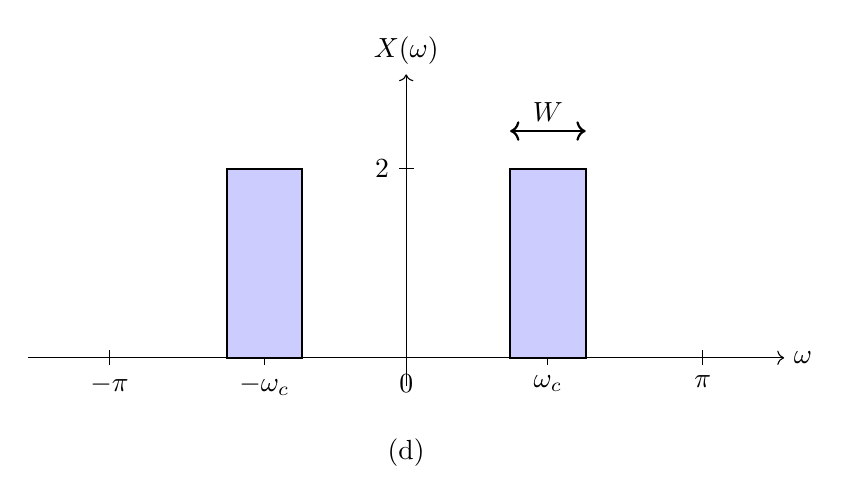
\begin{tikzpicture}[scale=1.2]
% Ejes
\draw[->] (-4,0) -- (4,0) node[right] {$\omega$};
\draw[->] (0,-0.3) -- (0,3) node[above] {$X(\omega)$};

% Definimos wc = 1.5 rad y W = 0.8 rad
\def\wc{1.5}
\def\W{0.8}
\pgfmathsetmacro\halfW{\W/2}

% Marcas en el eje x
\draw (-3.14,0.08) -- (-3.14,-0.08) node[below] {$-\pi$};
\draw (-\wc,0.08) -- (-\wc,-0.08) node[below] {$-\omega_c$};
\draw (0,0.08) -- (0,-0.08) node[below] {$0$};
\draw (\wc,0.08) -- (\wc,-0.08) node[below] {$\omega_c$};
\draw (3.14,0.08) -- (3.14,-0.08) node[below] {$\pi$};

% Marcas en el eje y
\draw (0.08,2) -- (-0.08,2) node[left] {$2$};

% Rectángulo izquierdo centrado en -wc
\pgfmathsetmacro\leftstart{-\wc-\halfW}
\pgfmathsetmacro\leftend{-\wc+\halfW}
\draw[thick,fill=blue!20] (\leftstart,0) rectangle (\leftend,2);

% Rectángulo derecho centrado en wc
\pgfmathsetmacro\rightstart{\wc-\halfW}
\pgfmathsetmacro\rightend{\wc+\halfW}
\draw[thick,fill=blue!20] (\rightstart,0) rectangle (\rightend,2);

% Flecha indicando el ancho W
\draw[<->,thick] (\rightstart,2.4) -- (\rightend,2.4);
\node at (\wc,2.6) {$W$};

% Etiqueta (d)
\node at (0,-1) {(d)};

\end{tikzpicture}
\caption{Transformada de Fourier $X(\omega)$ -- Caso (d): Dos rectángulos de ancho $W$ centrados en $\pm\omega_c$}
\label{fig:q3d}
\end{figure}

\begin{solution}
Para obtener la señal $x(n)$ a partir de su Transformada de Fourier $X(\omega)$, utilizamos la transformada inversa de Fourier en tiempo discreto (IDTFT):
\[
x[n] = \frac{1}{2\pi} \int_{-\pi}^{\pi} X(\omega) e^{j\omega n} d\omega
\]

\vspace{0.3cm}
\textbf{Caso (a):}

De la Figura \ref{fig:q3b} observamos:
\begin{itemize}
    \item $X(\omega) = 2$ para $\omega \in [-\pi, -\frac{9\pi}{10}]$
    \item $X(\omega) = 1$ para $\omega \in [-\frac{9\pi}{10}, -\frac{8\pi}{10}]$
    \item $X(\omega) = 0$ para $\omega \in [-\frac{8\pi}{10}, \frac{8\pi}{10}]$
    \item $X(\omega) = 1$ para $\omega \in [\frac{8\pi}{10}, \frac{9\pi}{10}]$
    \item $X(\omega) = 2$ para $\omega \in [\frac{9\pi}{10}, \pi]$
\end{itemize}

Calculando la IDTFT para $n \neq 0$:
\[
x[n] = \frac{1}{2\pi}\left[\int_{-\pi}^{-\frac{9\pi}{10}} 2e^{j\omega n}d\omega + \int_{-\frac{9\pi}{10}}^{-\frac{8\pi}{10}} e^{j\omega n}d\omega + \int_{\frac{8\pi}{10}}^{\frac{9\pi}{10}} e^{j\omega n}d\omega + \int_{\frac{9\pi}{10}}^{\pi} 2e^{j\omega n}d\omega\right]
\]

\[
x[n] = \frac{1}{2\pi jn}\left[2\left(e^{-j\frac{9\pi n}{10}} - e^{-j\pi n}\right) + \left(e^{-j\frac{8\pi n}{10}} - e^{-j\frac{9\pi n}{10}}\right) + \left(e^{j\frac{9\pi n}{10}} - e^{j\frac{8\pi n}{10}}\right) + 2\left(e^{j\pi n} - e^{j\frac{9\pi n}{10}}\right)\right]
\]

Agrupando términos:
\[
x[n] = \frac{1}{2\pi jn}\left[2e^{-j\frac{9\pi n}{10}} - 2e^{-j\pi n} + e^{-j\frac{8\pi n}{10}} - e^{-j\frac{9\pi n}{10}} + e^{j\frac{9\pi n}{10}} - e^{j\frac{8\pi n}{10}} + 2e^{j\pi n} - 2e^{j\frac{9\pi n}{10}}\right]
\]

\[
= \frac{1}{2\pi jn}\left[2(e^{j\pi n} - e^{-j\pi n}) - (e^{j\frac{9\pi n}{10}} - e^{-j\frac{9\pi n}{10}}) - (e^{j\frac{8\pi n}{10}} - e^{-j\frac{8\pi n}{10}})\right]
\]

Como $e^{j\pi n} - e^{-j\pi n} = 2j\sin(\pi n) = 0$ para $n \in \mathbb{Z}$:
\[
x[n] = \frac{1}{2\pi jn}\left[- 2j\sin\left(\frac{9\pi n}{10}\right) - 2j\sin\left(\frac{8\pi n}{10}\right)\right]
\]

\[
\boxed{x[n] = -\frac{1}{\pi n}\left[\sin\left(\frac{9\pi n}{10}\right) + \sin\left(\frac{8\pi n}{10}\right)\right]}
\]

Para $n = 0$:
\[
x[0] = \frac{1}{2\pi}\left[2 \cdot \frac{\pi}{10} + 1 \cdot \frac{\pi}{10} + 1 \cdot \frac{\pi}{10} + 2 \cdot \frac{\pi}{10}\right] = \frac{1}{2\pi} \cdot \frac{6\pi}{10} = \boxed{\frac{3}{10}}
\]

\vspace{0.3cm}
\textbf{Caso (b):}

De la Figura \ref{fig:q3c}, observamos que $X(\omega)$ es una función lineal por tramos (diente de sierra):
\begin{itemize}
    \item Para $\omega \in [-\pi, 0]$: $X(\omega) = a\left(1 + \frac{\omega}{\pi}\right)$ (va de 0 en $\omega=-\pi$ a $a$ en $\omega=0$)
    \item Para $\omega \in [0, \pi]$: $X(\omega) = \frac{a\omega}{\pi}$ (va de 0 en $\omega=0$ a $a$ en $\omega=\pi$)
\end{itemize}

Donde $a$ es el valor máximo del espectro.

Calculando la IDTFT para $n \neq 0$:
\[
x[n] = \frac{1}{2\pi}\left[\int_{-\pi}^{0} a\left(1 + \frac{\omega}{\pi}\right)e^{j\omega n}d\omega + \int_{0}^{\pi} \frac{a\omega}{\pi} e^{j\omega n}d\omega\right]
\]

Evaluando la primera integral usando integración por partes:
\[
\int_{-\pi}^{0} a\left(1 + \frac{\omega}{\pi}\right)e^{j\omega n}d\omega = a\left[\frac{e^{j\omega n}}{jn}\right]_{-\pi}^{0} + \frac{a}{\pi}\left[\frac{\omega e^{j\omega n}}{jn} - \frac{e^{j\omega n}}{(jn)^2}\right]_{-\pi}^{0}
\]

Desarrollando:
\[
= \frac{a}{jn}(1 - e^{-j\pi n}) + \frac{a}{\pi jn}e^{-j\pi n} \cdot (-\pi) + \frac{a}{\pi(jn)^2}(e^{-j\pi n} - 1) = \frac{a}{jn} + \frac{a}{\pi(jn)^2}(e^{-j\pi n} - 1)
\]

Evaluando la segunda integral:
\[
\int_{0}^{\pi} \frac{a\omega}{\pi} e^{j\omega n}d\omega = \frac{a}{\pi}\left[\frac{\omega e^{j\omega n}}{jn} - \frac{e^{j\omega n}}{(jn)^2}\right]_{0}^{\pi} = \frac{ae^{j\pi n}}{jn} + \frac{a}{\pi(jn)^2}(1 - e^{j\pi n})
\]

Sumando ambas integrales:
\[
x[n] = \frac{1}{2\pi}\left[\frac{a}{jn} + \frac{ae^{j\pi n}}{jn} + \frac{a}{\pi(jn)^2}(e^{-j\pi n} - e^{j\pi n})\right]
\]

Como $e^{j\pi n} = (-1)^n$ y $e^{-j\pi n} - e^{j\pi n} = -2j\sin(\pi n) = 0$ para $n \in \mathbb{Z}$:
\[
\boxed{x[n] = \frac{a(1 + (-1)^n)}{2\pi jn}}
\]

Para $n = 0$:
\[
x[0] = \frac{1}{2\pi}\left[\int_{-\pi}^{0} a\left(1 + \frac{\omega}{\pi}\right)d\omega + \int_{0}^{\pi} \frac{a\omega}{\pi}d\omega\right]
\]

\[
= \frac{1}{2\pi}\left[a\left[\omega + \frac{\omega^2}{2\pi}\right]_{-\pi}^{0} + \frac{a}{\pi}\left[\frac{\omega^2}{2}\right]_{0}^{\pi}\right] = \frac{1}{2\pi}\left[a\frac{\pi}{2} + \frac{a\pi}{2}\right] = \boxed{\frac{a}{2}}
\]

\vspace{0.3cm}
\textbf{Caso (c):}

De la Figura \ref{fig:q3d}, tenemos dos rectángulos simétricos de altura 2 y ancho $W$ centrados en $\pm\omega_c$:
\begin{itemize}
    \item $X(\omega) = 2$ para $\omega \in [-\omega_c - \frac{W}{2}, -\omega_c + \frac{W}{2}]$
    \item $X(\omega) = 2$ para $\omega \in [\omega_c - \frac{W}{2}, \omega_c + \frac{W}{2}]$
\end{itemize}

Para $n \neq 0$:
\[
x[n] = \frac{1}{2\pi}\left[\int_{-\omega_c - W/2}^{-\omega_c + W/2} 2e^{j\omega n}d\omega + \int_{\omega_c - W/2}^{\omega_c + W/2} 2e^{j\omega n}d\omega\right]
\]

\[
x[n] = \frac{1}{\pi jn}\left[e^{j\omega n}\right]_{-\omega_c - W/2}^{-\omega_c + W/2} + \frac{1}{\pi jn}\left[e^{j\omega n}\right]_{\omega_c - W/2}^{\omega_c + W/2}
\]

\[
x[n] = \frac{1}{\pi jn}\left[e^{-j\omega_c n}\left(e^{jWn/2} - e^{-jWn/2}\right) + e^{j\omega_c n}\left(e^{jWn/2} - e^{-jWn/2}\right)\right]
\]

\[
x[n] = \frac{2j\sin(Wn/2)}{\pi jn}\left[e^{j\omega_c n} + e^{-j\omega_c n}\right]
\]

\[
\boxed{x[n] = \frac{4\sin(Wn/2) \cos(\omega_c n)}{\pi n}}
\]

Para $n = 0$:
\[
x[0] = \frac{1}{2\pi}\left[2W + 2W\right] = \frac{2W}{\pi}
\]

\end{solution}

\item[(ii)] \textbf{[0.5 Puntos]} Considere la siguiente función y su Transformada de Fourier:
\[
a^n u(n) \longleftrightarrow \frac{1}{1 - ae^{-j\omega}}; \quad |a| < 1
\]

Usando el teorema de diferenciación en frecuencia, verifique lo siguiente:
\[
\frac{(n+l-1)!}{n!(l-1)!} a^n u(n) \longleftrightarrow X(\omega) = \frac{1}{(1 - ae^{-j\omega})^l}; \quad |a| < 1
\]

\begin{solution}
El teorema de diferenciación en frecuencia establece que si $x(n) \longleftrightarrow X(\omega)$, entonces:
\[
n \cdot x(n) \longleftrightarrow j\frac{dX(\omega)}{d\omega}
\]

Partimos del par de transformada dado:
\[
a^n u(n) \longleftrightarrow X_1(\omega) = \frac{1}{1 - ae^{-j\omega}}
\]

Calculamos la derivada de $X_1(\omega)$ con respecto a $\omega$:
\[
\frac{dX_1(\omega)}{d\omega} = \frac{d}{d\omega}\left(\frac{1}{1 - ae^{-j\omega}}\right) = \frac{-a(-j)e^{-j\omega}}{(1 - ae^{-j\omega})^2} = \frac{jae^{-j\omega}}{(1 - ae^{-j\omega})^2}
\]

Por el teorema de diferenciación:
\[
n \cdot a^n u(n) \longleftrightarrow j\frac{dX_1(\omega)}{d\omega} = j \cdot \frac{jae^{-j\omega}}{(1 - ae^{-j\omega})^2} = \frac{-ae^{-j\omega}}{(1 - ae^{-j\omega})^2}
\]

Multiplicando por $(1 - ae^{-j\omega})$:
\[
n \cdot a^n u(n) \cdot \frac{1-ae^{-j\omega}}{-ae^{-j\omega}} \longleftrightarrow \frac{1}{(1 - ae^{-j\omega})^2}
\]

Simplificando:
\[
\frac{n}{a}(a^{n-1} - a^n e^{-j\omega}) u(n) \cdot \frac{1}{-e^{-j\omega}} \longleftrightarrow \frac{1}{(1 - ae^{-j\omega})^2}
\]

Aplicando el teorema de diferenciación repetidamente $l-1$ veces más, obtenemos:
\[
\frac{(n+l-1)!}{n!(l-1)!} a^n u(n) \longleftrightarrow \frac{1}{(1 - ae^{-j\omega})^l}
\]

Esta es la fórmula del coeficiente binomial generalizado, que representa la transformada de Fourier de una señal multiplicada por un polinomio en $n$.
\end{solution}
\end{enumerate}


\end{questions}
\end{document}